\begin{section}{Motivation}

The High Luminosity LHC (HL-LHC) upgrade will offer unprecedented energies to explore for new physics, but it brings with it new complications that must be addressed by upgraded or additional detector hardware. Foremost among the new challenges posed by the HL-LHC is that higher luminosity means many more particles, which provides a far more complex picture to reconstruct for analysis. One such complexity is the increase in collision points, which is a key component of both offline and online reconstruction. With more particles colliding, collision points start to ``pile up'' on top of each other in space (this phenomena is aptly referred to as \textit{pile up}). Consequently, when reconstructing collisions into discrete ``events,'' one for each proton-proton collision, the reconstruction algorithm is unable to discern between one collision and many others that occurred in the same point in space. However, we know that these collisions occur at different \textit{times}, so adding timing information would certainly help reduce pileup. To this end, it has been proposed that a layer of silicon-based sensors, with sufficient timing resolutions, be placed around the parimeter -- surrounding the barrel and covering the endcap -- of the CMS detector, but the design and approval of such an upgrade is no simple task. From its conceptual inception to the finalization of its technical design, questions continually arise, so clear, cogent answers are constantly required, but since the detector has yet to be built, computer simulations are necessary to address these important concerns regarding the design and projected performance of the MTD.

\end{section}

\begin{section}{The Topolino Design}

The barrel and endcap layers (BTL and ETL respectively) of the MTD have rotational symmetries -- they are round -- while the sensors are rectangular. Thus, correctly fitting the rectangular sensors to the circular space allotted on the endcaps becomes a complicated exercise in geometric optimization, while including space for all of the required circuitry, wiring, and cooling systems imposes complicated physical constraints. For the BTL, the design is fairly simple: long trays of sensors may be laid along the axis of the barrel, maintaining its cylindrical symmetry. The ETL was not so simple to cover, but one design was arrived at, named ``Topolino'' (Mickey Mouse in Italian) by its inventor, where the ETL is divided into four ninety-degree wedges. The front of each wedge is tiled with parallel strips of sensors that continue up until the the edge of the endcap. The back of the same wedge is similarly covered, but the sensors are horizontally offset to cover the gaps left by the readout electronics on the front. Each wedge is covered in this way, then placed such that the sensors in each is perpendicular to its neighboring wedges. See Figure \ref{fig:topolino} for a detailed visualization of the proposed design.

\end{section}

\begin{section}{Rendering the Detector}

Detector physics simulation begins with a simulation of the detector, but for answers to questions about the MTD's design and performance, verbose considerations of minute physical interactions are, at the moment, unnecessary. Therefore, though more complex tools offer more accurate physics, a simple rendering of each sensor's position is space is sufficient. However, the simulation must also be configurable, so assembling the it by hand, like most 3D-modeling software requires, was neither an entertaining, nor efficient solution. Instead, OpenSCAD, a C-like programming language that allows for simple, modular construction of three-dimensional models, was selected.

To algorithmically implement the Topolino design, fundamental rules that govern the layout had to be established. First, neither the sensors, nor the space allotted for their circuitry, could be allowed to hang over the perimeter of the endcap. Second, sensors are most easily assembled and placed as modules, so the detector must be tiled by \textit{groups} of sensors. Finally, the service modules -- the ``circuitry'' for which space has already been allotted -- are designed to service sensors on both sides, so sensors should (generally) be placed as such, resulting in a neat grid. With these rules in mind, an algorithm parses the x-axis in increments equal to the width of a sensor module, then places sensors by their lower, left-hand (closest to origin) corners, so long as their placement does not violate any of the previously stated rules. One wedge is tiled in this way with the sensors on its reverse side simply placed starting from a given displacement from the origin such that the holes left by the spacing for readout electronics. The rest of the endcap is covered by simply taking this wedge, then placing orthogonally-rotated copies until the entire surface is covered.

\begin{figure}[htb]
\begin{center}
\subfloat[Rendered with no mounting disk to show coverage of electronics gaps.]      {
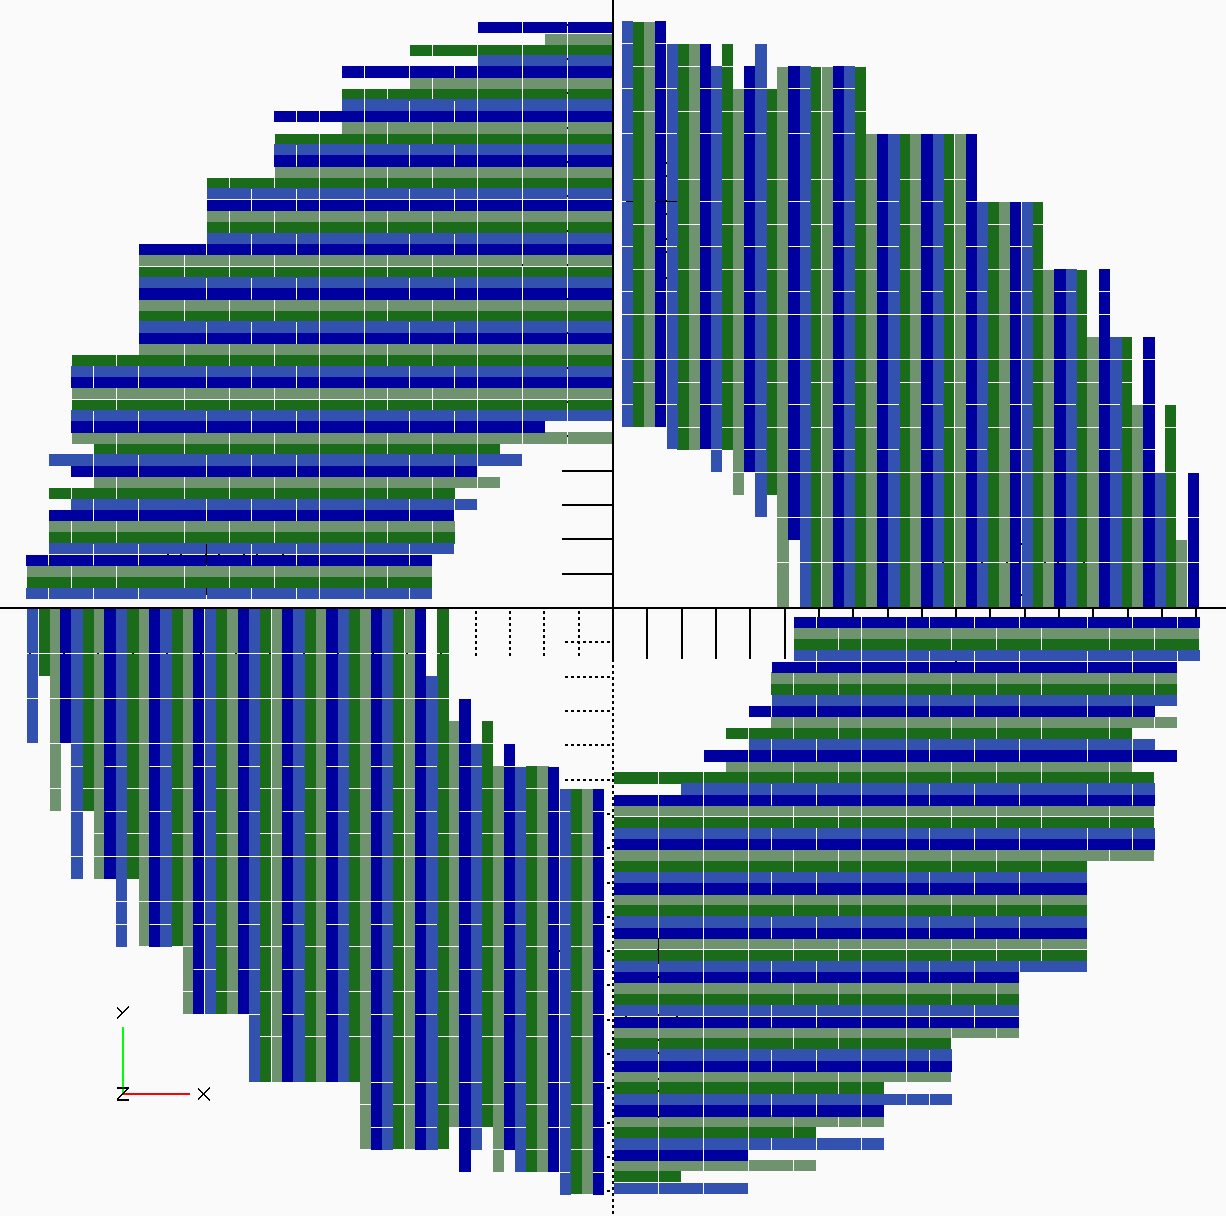
\includegraphics[width=.5\linewidth]{Dissertation/fig/topolino-nodisk.png}
}
\\
\subfloat[Front of one full disk.]      {
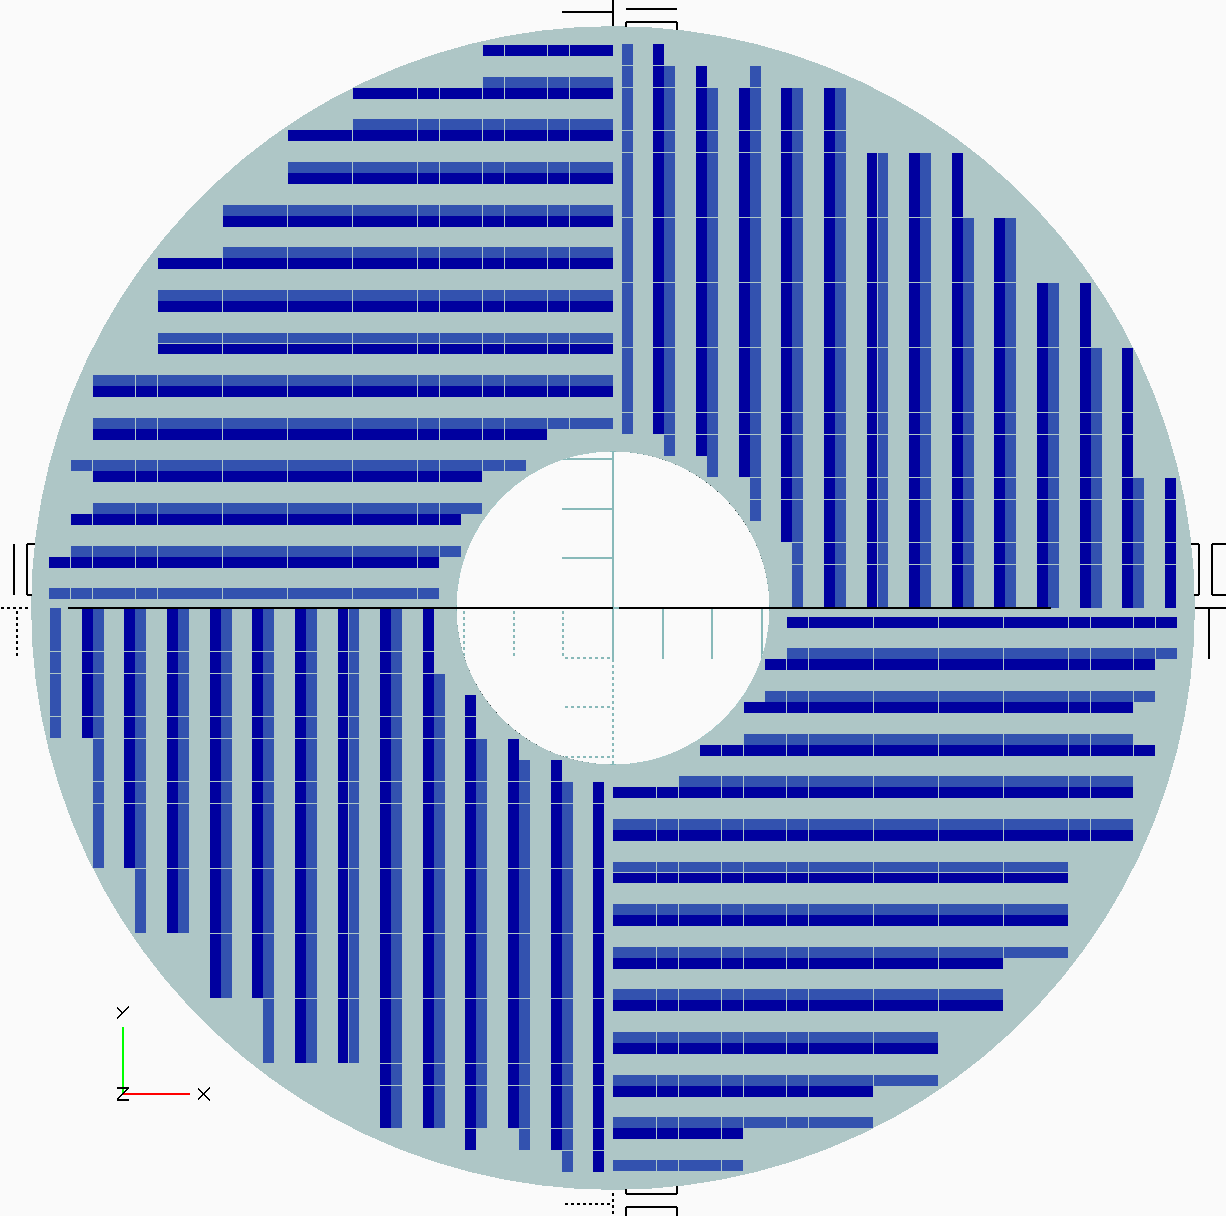
\includegraphics[width=.25\linewidth]{Dissertation/fig/topolino-front.png}
}\quad
\subfloat[Back of one full disk.]      {
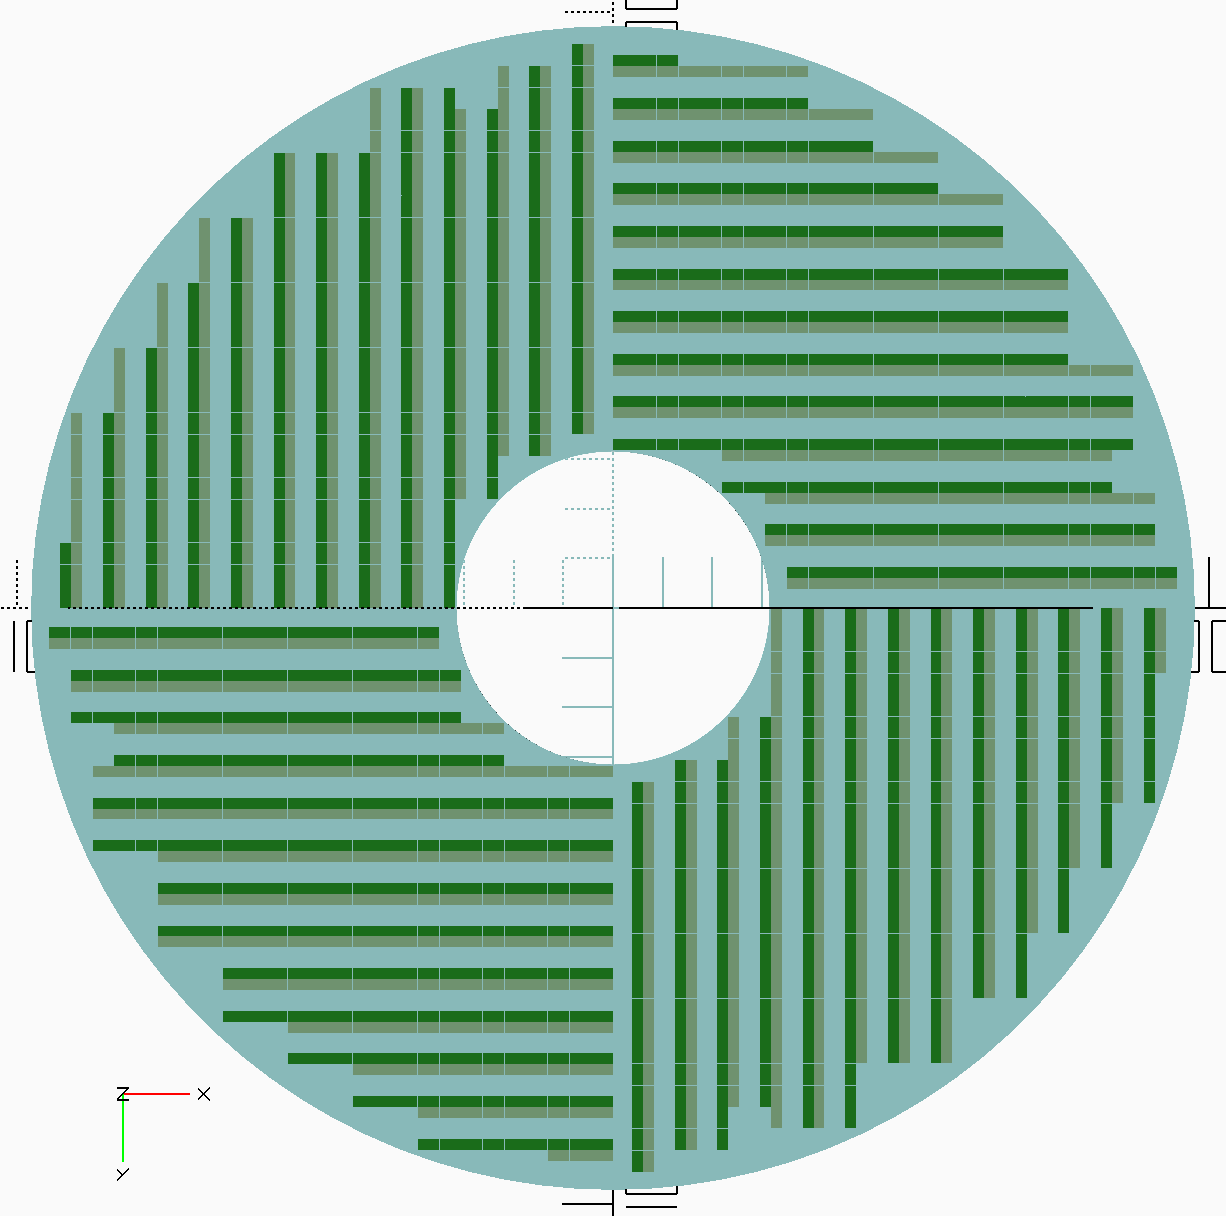
\includegraphics[width=.25\linewidth]{Dissertation/fig/topolino-back.png}
}
\end{center}
\caption{The ``topolino'' design.}
\label{fig:topolino}
\end{figure}

\end{section}

\begin{section}{Simulating Performance}
\begin{subsection}{Pre-processing}
The three-dimensional model of the MTD can be exported as a Standard Tessellation Language (STL) file. During the export process, each independent object -- say, a single sensor which is represented as a thin rectangular prism -- is broken down into each of its constituent faces. Then, undergoes the tessellation process, wherein the face considered is broken into some optimal number of constituent triangles (triangles typically are used for simplicity of later calculations). The \textit{vertices} of each of these triangles, hereafter referred to as \textit{polygons}, are then written to the STL file, in a clockwise order relative to the origin. It is important to note that this guarantees that the \textit{facet normal} vector -- that is, the vector is orthogonal to the surface of the polygon with a magnitude equal to the are of the polygon -- always points outwards with respect to the origin.
\end{subsection}
\begin{subsection}{Hit Detection Algorithm}
Now, before the simulation is generally discussed, the algorithm by which an intersection between a point and a polygon is determined should first be outlined, since it is the core of the simulation but is otherwise only tangentially important to the overall process. Consider a triangle in three-space, namely a set of three vectors $\vec{v}_1, \vec{v}_2, \vec{v}_3$ with facet normal $\hat{n}$, normalized such that $|\hat{n}| = 1$, pointing outwards relative to the origin. Then, suppose there exists a point $\vec{a}$ somewhere in three-space (see Figure \ref{fig:setup} for a visual representation of this setup). First, the coordinate system must be rotated into the plane of the polygon (in order to account for both the azimuthal symmetry of the BTL and radial symmetry of the ETL). One basis vector, arbitrarily chosen to be $\hat{e}_3'$, is already given by the facet normal vector. Another, now chosen to be $\hat{e}_{1}'$, is given by the original $\hat{e}_3$ vector (this is $\hat{z}$ is the CMS coordinate system; see Appendix \ref{appendix:a} for more information). With two basis vectors determined, the third is simply given by the cross product $\hat{e}_3'\times\hat{e}_1'$, assuming they are already normalized (again, see Figure \ref{fig:setup}). From this new set of basis vectors $\hat{e}_i'$, still represented in the original basis, a matrix $R$ can be constructed to translate any arbitrary vector into the primed coordinate system:

\begin{equation}
    \hat{e}_i' = \begin{pmatrix} x_i \\ y_i \\ z_i \end{pmatrix}
    \rightarrow
    R \equiv \begin{pmatrix} 
        x_1 & y_1 & z_1 \\
        x_2 & y_2 & z_2 \\
        x_3 & y_3 & z_3
    \end{pmatrix}
\end{equation}

\noindent The point $\vec{a}$ and vertices $\vec{v}_i$ are translated into the primed coordinate system such that $R\vec{a} = \vec{a}'$ and $R\vec{v}_i = \vec{v}_{i}'$. Then, the $\hat{e}_3'$ coordinates of $\vec{a}'$ and $\vec{v}_i'$ are set to zero, ensuring that all points considered are in the same plane parallel to that spanned by the polygon. Now, the vector from the point $\vec{a}'$ to the vertex $\vec{v}_{i}'$ is defined as $\vec{d}_{i}' \equiv \vec{v}_{i}'-\vec{a}'$. Finally, the following cross products are defined:

\begin{equation}
    \vec{C}_{i}' \equiv \epsilon_{ijk}(\vec{d}_{j}'\times\vec{d}_{k}')
\end{equation}

\noindent In words, the vectors $\vec{C}_{i}'$ are the cross products between adjacent vectors $\vec{d}_{j}'$, $\vec{d}_{k}'$ taken in cyclical permutations, as dictated by the Levi-Cevita symbol $\epsilon_{ijk}$. More importantly, however, each vector $\vec{C}_{i}'$ must be \textit{parallel} to the facet normal vector, which is $\hat{e}_{3}'$ in the primed coordinate system, if it lies \textit{inside} of the polygon. This is because the angles between each vector $\vec{d}_{i}'$ must add up to 180 degrees inside the polygon or 360 degrees outside by geometric constraint, so the angle between two vectors $\vec{d}_{i}'$, $\vec{d}_{j}'$ has an \textit{upper limit} of 180 degrees inside of the triangle and 360 degrees outside. Now, the cross product between these vectors will point one way (here, the positive $\hat{e}_3'$ direction) if the angle between them is less than 180 degrees or exactly anti-parallel (the $-\hat{e}_3'$ direction) otherwise, so if all $\vec{C}_{i}'$ are \textit{greater than} zero, $\vec{a}$ must be inside of the polygon, otherwise, it can immediately determined that $\vec{a}$ is outside. Put concisely, point $\vec{a}$ intersects the polygon given by $\vec{v}_1, \vec{v}_2, \vec{v}_3$ and facet normal $\hat{n}$ if and only if $\vec{C}_{i}' > 0$ where $i\in[1,2,3]$.

\begin{figure}[htb]
\begin{center}

\subfloat[Original]      {
\tdplotsetmaincoords{60}{110}
\begin{tikzpicture}[scale=3,tdplot_main_coords]
 
  % variables
  % theta, phi for a
  \def\rvec{.8}
  \def\thetavec{30}
  \def\phivec{345}
  % theta, phi for v1
  \def\rvecone{1.0}
  \def\thetavecone{15}
  \def\phivecone{90}
  % theta, phi for v2
  \def\rvectwo{1.0}
  \def\thetavectwo{74}
  \def\phivectwo{54}
  % theta, phi for v3
  \def\rvecthree{0.8}
  \def\thetavecthree{74}
  \def\phivecthree{90}
  % theta, phi for n
  \def\rvecfour{.7}
  \def\thetavecfour{37}
  \def\phivecfour{72}
 
  % axes
  \coordinate (O) at (0,0,0);
  \draw[thick,->] (0,0,0) -- (1,0,0) node[anchor=north east]{$\hat{e}_1$};
  \draw[thick,->] (0,0,0) -- (0,1,0) node[anchor=north west]{$\hat{e}_2$};
  \draw[thick,->] (0,0,0) -- (0,0,1) node[anchor=south]{$\hat{e}_3$};
 
  % a
  \tdplotsetcoord{P}{\rvec}{\thetavec}{\phivec}
  \draw[-stealth,black] (O)  -- (P) node[above right] {$\vec{a}$};
  \draw[dashed,black]   (O)  -- (Pxy);
  \draw[dashed,black]   (P)  -- (Pxy);
  % n
  \tdplotsetcoord{N}{\rvecfour}{\thetavecfour}{\phivecfour}
  \draw[-stealth,black] (O)  -- (N) node[above right] {$\hat{n}$};
  \draw[dashed,black]   (O)  -- (Nxy);
  \draw[dashed,black]   (N)  -- (Nxy);
  % v1
  \tdplotsetcoord{A}{\rvecone}{\thetavecone}{\phivecone}
  \draw[-stealth,red] (O)  -- (A) node[above right] {$\vec{v}_1$};
  \draw[dashed,red]   (O)  -- (Axy);
  \draw[dashed,red]   (A)  -- (Axy);
  \draw[dashed,red]   (Ay) -- (Axy);
  % v2
  \tdplotsetcoord{B}{\rvectwo}{\thetavectwo}{\phivectwo}
  \draw[-stealth,green] (O)  -- (B) node[above right] {$\vec{v}_2$};
  \draw[dashed,green]   (O)  -- (Bxy);
  \draw[dashed,green]   (B)  -- (Bxy);
  \draw[dashed,green]   (By) -- (Bxy);
  % v3
  \tdplotsetcoord{C}{\rvecthree}{\thetavecthree}{\phivecthree}
  \draw[-stealth,blue] (O)  -- (C) node[above right] {$\vec{v}_3$};
  \draw[dashed,blue]   (O)  -- (Cxy);
  \draw[dashed,blue]   (C)  -- (Cxy);
  \draw[dashed,blue]   (Cy) -- (Cxy);
 
\end{tikzpicture}
}\quad
\subfloat[Primed]      {
\tdplotsetmaincoords{60}{110}
\begin{tikzpicture}[scale=3,tdplot_main_coords]
 
  % variables
  % theta, phi for a
  \def\rvec{.8}
  \def\thetavec{30}
  \def\phivec{345}
  % theta, phi for v1
  \def\rvecone{1.0}
  \def\thetavecone{15}
  \def\phivecone{90}
  % theta, phi for v2
  \def\rvectwo{1.0}
  \def\thetavectwo{74}
  \def\phivectwo{54}
  % theta, phi for v3
  \def\rvecthree{0.8}
  \def\thetavecthree{74}
  \def\phivecthree{90}
  % theta, phi for n
  \def\rvecfour{.7}
  \def\thetavecfour{37}
  \def\phivecfour{72}
  % theta, phi for e2
  \def\rvecfive{1.0}
  \def\thetavecfive{-53}
  \def\phivecfive{90}
 
  % axes
  \coordinate (O) at (0,0,0);
  \draw[thick,->] (0,0,0) -- (1,0,0) node[anchor=north east]{$\hat{e}_{1}'$};
  \tdplotsetcoord{E}{\rvecfive}{\thetavecfive}{\phivecfive}
  \draw[thick,->] (0,0,0) -- (E) node[anchor=north west]{$\hat{e}_{2}'$};
  \tdplotsetcoord{E}{\rvecfour}{\thetavecfour}{\phivecfour}
  \draw[thick,->] (0,0,0) -- (E) node[anchor=south]{$\hat{e}_{3}'$};
 
  % a
  \tdplotsetcoord{P}{\rvec}{\thetavec}{\phivec}
  \draw[-stealth,black] (O)  -- (P) node[above right] {$\vec{a}$};
  \draw[dashed,black]   (O)  -- (Pxy);
  \draw[dashed,black]   (P)  -- (Pxy);
  % v1
  \tdplotsetcoord{A}{\rvecone}{\thetavecone}{\phivecone}
  \draw[-stealth,red] (O)  -- (A) node[above right] {$\vec{v}_1$};
  \draw[dashed,red]   (O)  -- (Axy);
  \draw[dashed,red]   (A)  -- (Axy);
  \draw[dashed,red]   (Ay) -- (Axy);
  % v2
  \tdplotsetcoord{B}{\rvectwo}{\thetavectwo}{\phivectwo}
  \draw[-stealth,green] (O)  -- (B) node[above right] {$\vec{v}_2$};
  \draw[dashed,green]   (O)  -- (Bxy);
  \draw[dashed,green]   (B)  -- (Bxy);
  \draw[dashed,green]   (By) -- (Bxy);
  % v3
  \tdplotsetcoord{C}{\rvecthree}{\thetavecthree}{\phivecthree}
  \draw[-stealth,blue] (O)  -- (C) node[above right] {$\vec{v}_3$};
  \draw[dashed,blue]   (O)  -- (Cxy);
  \draw[dashed,blue]   (C)  -- (Cxy);
  \draw[dashed,blue]   (Cy) -- (Cxy);
 
\end{tikzpicture}
}

\end{center}
\caption{Coordinate systems used.}
\label{fig:setup}
\end{figure}

\begin{figure}[htb]
\begin{center}

\subfloat[Inside]      {
\tdplotsetmaincoords{60}{110}
\begin{tikzpicture}[scale=3,tdplot_main_coords]
 
  % variables
  % theta, phi for v1
  \def\rvecone{1.0}
  \def\thetavecone{90}
  \def\phivecone{90}
  % theta, phi for v2
  \def\rvectwo{1.0}
  \def\thetavectwo{90}
  \def\phivectwo{54}
  % theta, phi for v3
  \def\rvecthree{0.8}
  \def\thetavecthree{90}
  \def\phivecthree{270}
 
  % axes
  \coordinate (O) at (0.2,-0.3,0);
  \draw[thick,->] (0,0,0) -- (1,0,0) node[anchor=north east]{$\hat{e}_1'$};
  \draw[thick,->] (0,0,0) -- (0,1,0) node[anchor=north west]{$\hat{e}_2'$};
  \draw[thick,->] (0,0,0) -- (0,0,1) node[anchor=south]{$\hat{e}_3'$};

  \draw plot [mark=*, mark size=0.5] coordinates{(0.2,-0.3,0)};
  % a
  \draw[-stealth,black] (0,0,0) -- (0.2,-0.3,0) node[above right]{$\vec{a}'$};
  % d1
  \tdplotsetcoord{A}{\rvecone}{\thetavecone}{\phivecone}
  \draw[-stealth,red] (O)  -- (A) node[above right] {$\vec{d}_{1}'$};
  % d2
  \tdplotsetcoord{B}{\rvectwo}{\thetavectwo}{\phivectwo}
  \draw[-stealth,green] (O)  -- (B) node[above right] {$\vec{d}_{2}'$};
  % d3
  \tdplotsetcoord{C}{\rvecthree}{\thetavecthree}{\phivecthree}
  \draw[-stealth,blue] (O)  -- (C) node[above right] {$\vec{d}_{3}'$};
  % d3->d1
  \tdplotdrawarc[thick,->]{(O)}{0.4}{246}{99}
  {anchor=north}{};
  % d1->d2
  \tdplotdrawarc[thick,->]{(O)}{0.4}{99}{68}
  {anchor=north}{};
  % d2->d3
  \tdplotdrawarc[thick,->]{(O)}{0.4}{68}{-114}
  {anchor=north}{};
 
\end{tikzpicture}
}\quad
\subfloat[Outside]      {
\tdplotsetmaincoords{60}{110}
\begin{tikzpicture}[scale=3,tdplot_main_coords]
 
  % variables
  % theta, phi for v1
  \def\rvecone{1.0}
  \def\thetavecone{90}
  \def\phivecone{90}
  % theta, phi for v2
  \def\rvectwo{1.0}
  \def\thetavectwo{90}
  \def\phivectwo{54}
  % theta, phi for v3
  \def\rvecthree{0.8}
  \def\thetavecthree{90}
  \def\phivecthree{270}
 
  % axes
  \coordinate (O) at (-0.75,0,0);
  \draw[thick,->] (0,0,0) -- (1,0,0) node[anchor=north east]{$\hat{e}_1'$};
  \draw[thick,->] (0,0,0) -- (0,1,0) node[anchor=north west]{$\hat{e}_2'$};
  \draw[thick,->] (0,0,0) -- (0,0,1) node[anchor=south]{$\hat{e}_3'$};

  \draw plot [mark=x, mark size=1] coordinates{(-0.75,0,0)};
  % a
  \draw[-stealth,black] (0,0,0) -- (-0.75,0,0) node[above right]{$\vec{a}'$};
  % d1
  \tdplotsetcoord{A}{\rvecone}{\thetavecone}{\phivecone}
  \draw[-stealth,red] (O)  -- (A) node[above right] {$\vec{d}_{1}'$};
  % d2
  \tdplotsetcoord{B}{\rvectwo}{\thetavectwo}{\phivectwo}
  \draw[-stealth,green] (O)  -- (B) node[above right] {$\vec{d}_{2}'$};
  % d3
  \tdplotsetcoord{C}{\rvecthree}{\thetavecthree}{\phivecthree}
  \draw[-stealth,blue] (O)  -- (C) node[above right] {$\vec{d}_{3}'$};
  % d3->d1
  \tdplotdrawarc[thick,->,dashed]{(O)}{0.5}{311}{54}
  {anchor=north}{};
  % d1->d2
  \tdplotdrawarc[thick,->]{(O)}{0.5}{54}{30}
  {anchor=north}{};
  % d2->d3
  \tdplotdrawarc[thick,->]{(O)}{0.5}{30}{-51}
  {anchor=north}{};
 
\end{tikzpicture}
}

\end{center}
\caption{Vectors from hit position to vertices.}
\label{fig:vectors}
\end{figure}

\end{subsection}
\begin{subsection}{Post-processing}
The STL representation of the MTD and a text file containing the kinematics of many thousands of simulated particle trajectories is now input to a Python program that operates as follows: for each trajectory in the trajectory file, parse over every polygon in the STL file and check if the trajectory intersects the polygon using the algorithm described previously; if true, save some kinematics of the trajectory including the hit position; else, continue. This is, in essence, how many ``ray tracing'' algorithms function\cite{raytrace}, which calculate effects like lighting for computer graphics. Ray tracing is a slow process, which is why graphics seen in movies are pre-rendered and far more detailed and realistic than graphics computed in real time, though recent developments are making real-time, brute-force ray tracing more feasible. However, such technology was neither present nor necessary for this simulation. Instead, the Condor\cite{condor} system on the Tier 2 computing center at UC San Diego was used to run the algorithm over approximately 250,000 trajectories. As a result, plots accurate up to the millimeter scale may be produced to study the efficiency of the entire MTD for a dynamic range of geometries. An example of the simulation's output is shown in Figure \ref{fig:chronoplots}.

\begin{figure}[htb]
\begin{center}
\subfloat[]      {
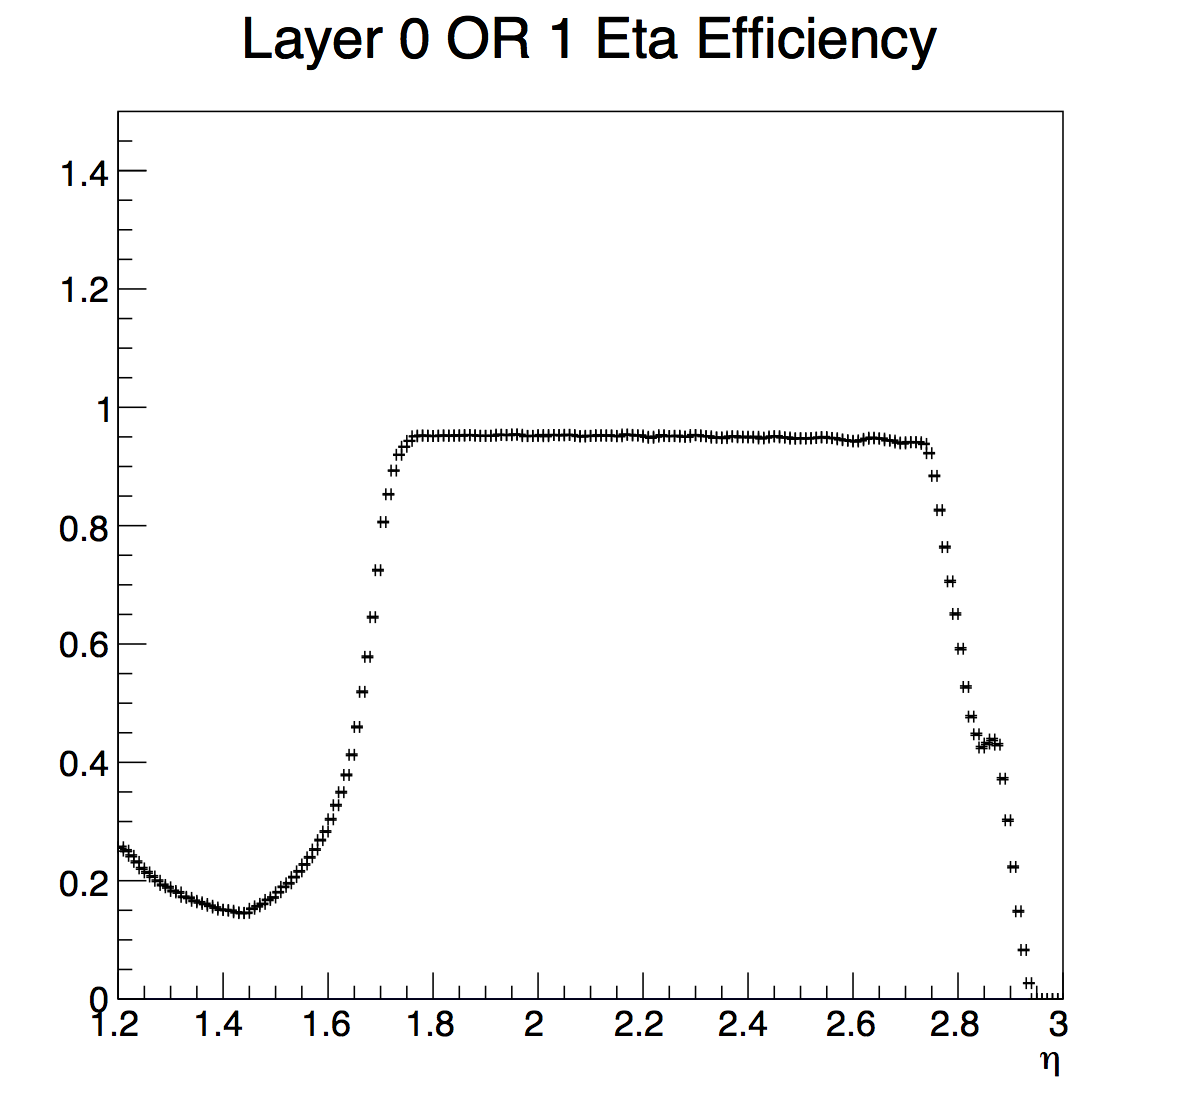
\includegraphics[width=.25\linewidth]{Dissertation/fig/DiskEtaEff01-1190mm.png}
}\quad
\subfloat[]      {
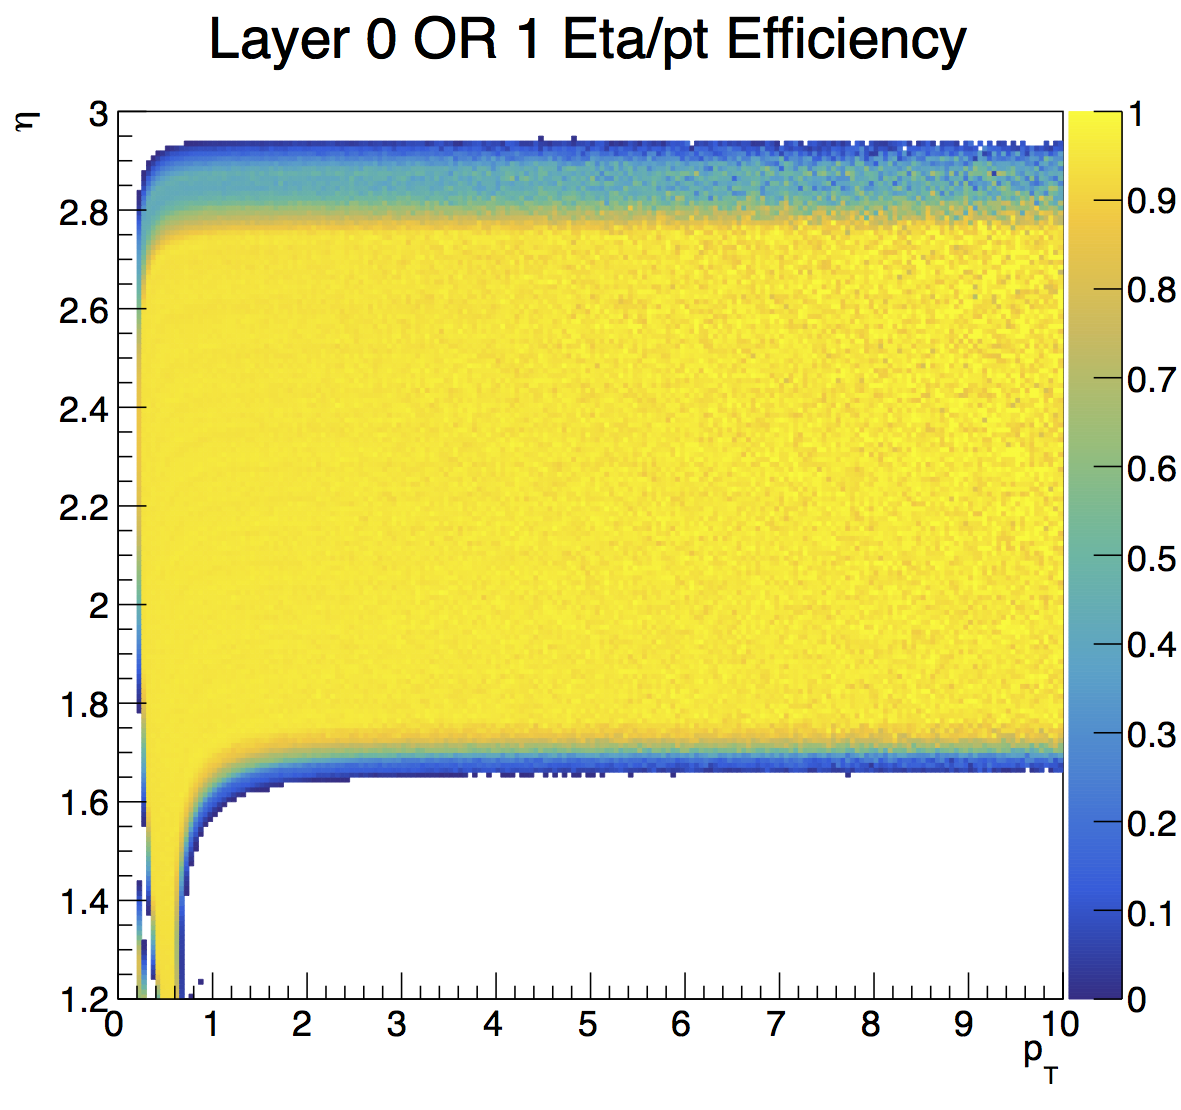
\includegraphics[width=.25\linewidth]{Dissertation/fig/DiskEtaPtEff01-1190mm.png}
}\\
\subfloat[]      {
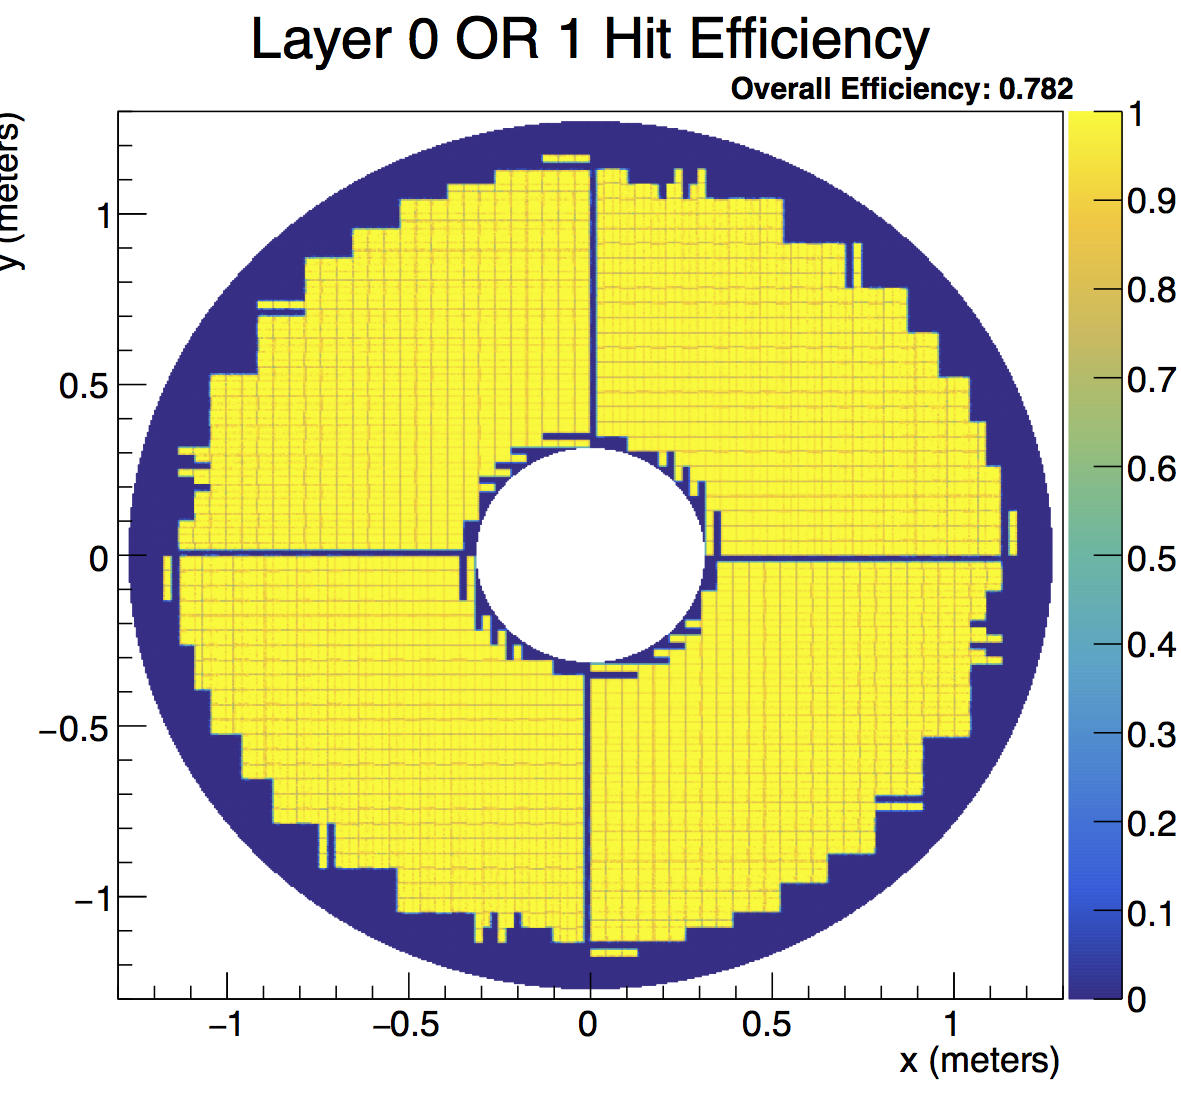
\includegraphics[width=.25\linewidth]{Dissertation/fig/LayerHitEff01-1190mm.png}
}\quad
\subfloat[]      {
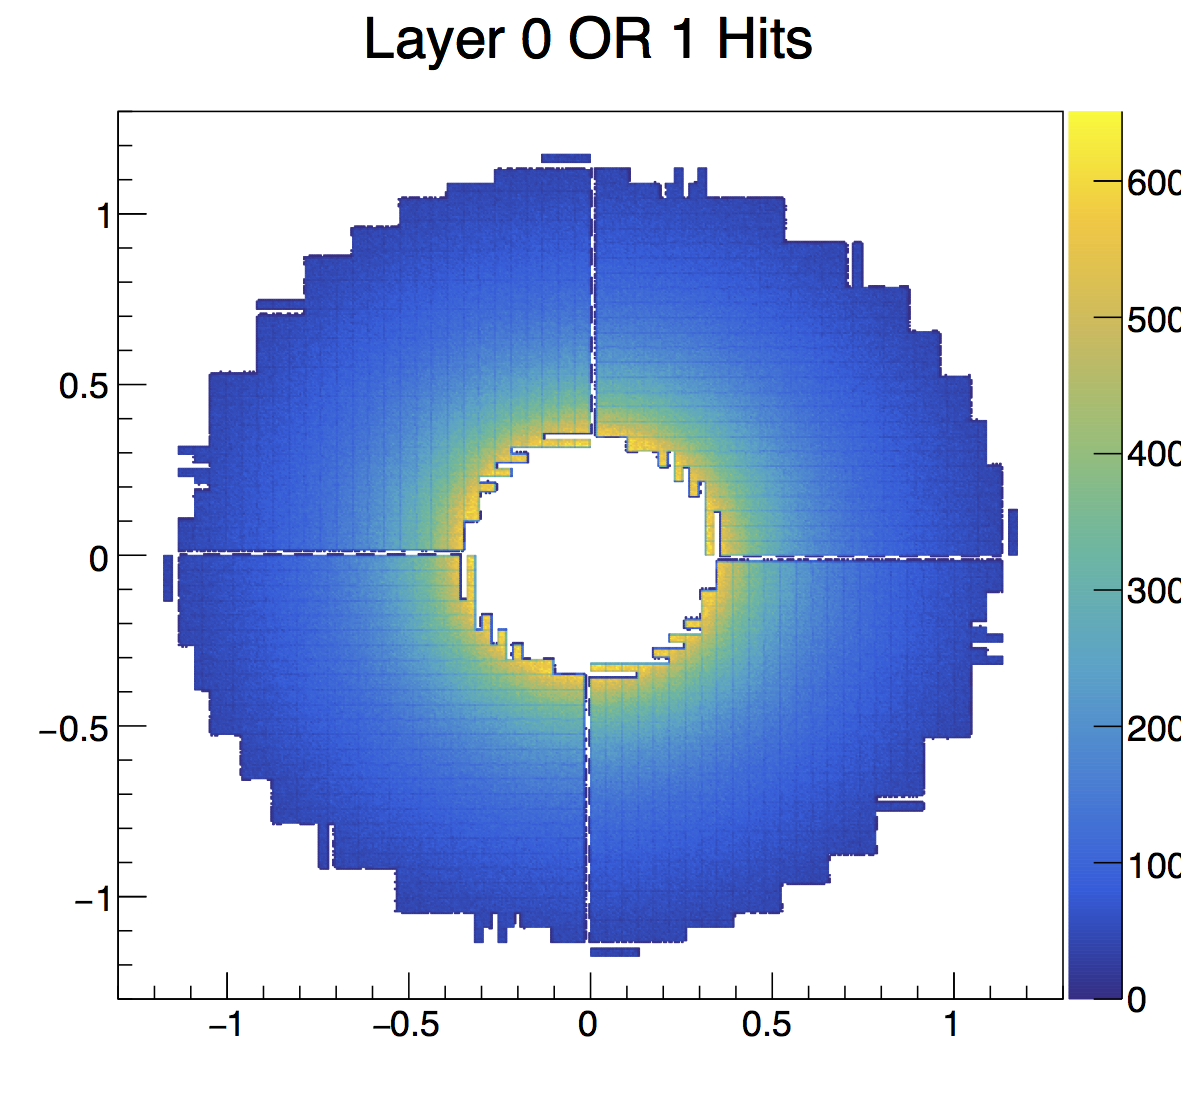
\includegraphics[width=.25\linewidth]{Dissertation/fig/LayerHits01-1190mm.png}
}
\end{center}
\caption{Efficiency plots produced using simulation data for the ETL with a 1190mm outer radius and 315mm inner radius following the Topolino design.}
\label{fig:chronoplots}
\end{figure}

\end{subsection}
\end{section}